% !Mode:: "TeX:UTF-8"
% !TEX program  = pdflatex
\documentclass[a4paper]{article}

% import settings, modify the number of homework in this file

\usepackage[T1]{fontenc}
\usepackage{amsmath, amssymb, amsthm}
% amsmath: equation*, amssymb: mathbb, amsthm: proof
\usepackage{moreenum}
\usepackage{mathtools}
\usepackage{url}
\usepackage{graphicx}
\usepackage{subcaption}
\usepackage{booktabs} 
\usepackage[mathcal]{eucal}
\usepackage{dsfont}
\usepackage{geometry}
\geometry{left=30mm,right=30mm,	top=42mm, bottom=33mm}

\usepackage[numbered,framed]{matlab-prettifier}
\lstset{
	style              = Matlab-editor,
	captionpos         =b,
	basicstyle         = \mlttfamily,
	escapechar         = ",
	mlshowsectionrules = true,
}

% set the homework count number
\usepackage[thehwcnt = 1]{iidef}

\newcommand\dif{\text{d}}
\newcommand\no{\noindent}
\newcommand\dis{\displaystyle}
\newcommand\ls{\leqslant}
\newcommand\gs{\geqslant}

\newcommand\limit{\dis\lim\limits}
\newcommand\limn{\dis\lim\limits_{n\to\infty}}
\newcommand\limxz{\dis\lim\limits_{x\to0}}
\newcommand\limxi{\dis\lim\limits_{x\to\infty}}
\newcommand\limxpi{\dis\lim\limits_{x\to+\infty}}
\newcommand\limxni{\dis\lim\limits_{x\to-\infty}}
\newcommand\limtpi{\dis\lim\limits_{t\to+\infty}}
\newcommand\limtni{\dis\lim\limits_{t\to-\infty}}

\newcommand\sumn{\dis\sum\limits_{n=1}^{\infty}}
\newcommand\sumnz{\dis\sum\limits_{n=0}^{\infty}}

\newcommand\sumi{\dis\sum\limits_{i=1}^{\infty}}
\newcommand\sumiz{\dis\sum\limits_{i=0}^{\infty}}
\newcommand\sumin{\dis\sum\limits_{i=1}^{n}}
\newcommand\sumizn{\dis\sum\limits_{i=0}^{n}}

\newcommand\sumk{\dis\sum\limits_{k=1}^{\infty}}
\newcommand\sumkz{\dis\sum\limits_{k=0}^{\infty}}
\newcommand\sumkn{\dis\sum\limits_{k=0}^n}
\newcommand\sumkfn{\dis\sum\limits_{k=1}^n}

\newcommand\pzx{\dis\frac{\partial z}{\partial x}}
\newcommand\pzy{\dis\frac{\partial z}{\partial y}}

\newcommand\pfx{\dis\frac{\partial f}{\partial x}}
\newcommand\pfy{\dis\frac{\partial f}{\partial y}}

\newcommand\pzxx{\dis\frac{\partial^2 z}{\partial x^2}}
\newcommand\pzxy{\dis\frac{\partial^2 z}{\partial x\partial y}}
\newcommand\pzyx{\dis\frac{\partial^2 z}{\partial y\partial x}}
\newcommand\pzyy{\dis\frac{\partial^2 z}{\partial y^2}}

\newcommand\pfxx{\dis\frac{\partial^2 f}{\partial x^2}}
\newcommand\pfxy{\dis\frac{\partial^2 f}{\partial x\partial y}}
\newcommand\pfyx{\dis\frac{\partial^2 f}{\partial y\partial x}}
\newcommand\pfyy{\dis\frac{\partial^2 f}{\partial y^2}}

\newcommand\intzi{\dis\int_{0}^{+\infty}}
\newcommand\intd{\dis\int}
\newcommand\intab{\dis\int_a^b}

\newcommand{\degree}{^\circ}

\newcommand\ma{\mathcal{A}}
\newcommand\mb{\mathcal{B}}
\newcommand\mc{\mathcal{C}}
\newcommand\me{\mathcal{E}}
\newcommand\mg{\mathcal{g}}

\newcommand\mcc{\mathbb{C}}
\newcommand\mrr{\mathbb{R}}
\newcommand\mzz{\mathbb{Z}}

\newcommand\mx{\bf{x}}
\newcommand\mX{\bf{X}}
\newcommand\my{\bf{y}}
\newcommand\mY{\bf{Y}}
%%=============================================

%%=====定义新数学符号===============================
\DeclareMathOperator{\sgn}{sgn}
\DeclareMathOperator{\arccot}{arccot}
\DeclareMathOperator{\arccosh}{arccosh}
\DeclareMathOperator{\arcsinh}{arcsinh}
\DeclareMathOperator{\arctanh}{arctanh}
\DeclareMathOperator{\arccoth}{arccoth}
\DeclareMathOperator{\grad}{\bf{grad}}
%\DeclareMathOperator{\argmax}{argmax}
%\DeclareMathOperator{\argmin}{argmin}
%\DeclareMathOperator{\diag}{diag}
\DeclareMathOperator{\csign}{csign}
%===============================================

\thecourseinstitute{Harbin Institute of Technology, ShenZhen}
\thecoursename{Operations Research}
\theterm{Fall 2019}
\hwname{Homework}

\begin{document}
\courseheader
\name{JingXuan Yang, SZ160310217}

\begin{enumerate}
  \setlength{\itemsep}{3\parskip}

% first exercise
  \item Label each of the following statements about linear programming problems as true or false.
  \begin{enumerate}
  	\item  For minimization problems, if the objective function evaluated at a CPF solution is no larger than its value at every adjacent CPF solution then that solution is optimal.
  	\begin{solution}
  			True
  	\end{solution}
  	
  	\item Only CPF solutions can be optimal, so the number of optimal solutions cannot exceed the number of CPF solutions.
  	\begin{solution}
  	False
  	\end{solution}  	
  	
  	\item If multiple optimal solutions exist, then an optimal CPF solution may have an adjacent CPF solution that also is optimal (the same value of $Z$).
  	\begin{solution}
  		True
  	\end{solution}
  	
  \end{enumerate}
  
%  \begin{figure}[htbp]
%  	\centering
%  	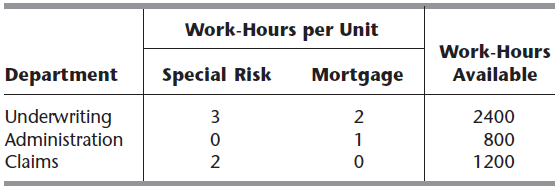
\includegraphics[width = 0.5\textwidth]{fig3-1-9}
%  \end{figure}  

% second excerise
  \item Solve the following problem by the simplex method in tabular form.
  
  Maximize $$ Z=2x_1-x_2+x_3$$
  subject to
  \begin{equation*}
	\begin{aligned}
 		3x_1+x_2+x_3&\ls 6\\
 		x_1-x_2+2x_3&\ls 1\\
 		x_1+x_2-x_3&\ls 2\\
 		x_1,\ x_2,\ x_3&\gs 0\\
  \end{aligned}
  \end{equation*}
  \begin{solution}
  	Use the following Tab.\ref{tab1} to solve this problem.
  	\begin{table}[h]
  		\centering
  		\caption{Simplex tableaux}
  		\label{tab1}
  		\begin{tabular}{ccccccccccc}
  			\toprule[1.5pt]
  			            Iteration&Basic Variable    &Eq.  &$Z$  &$x_1$&$x_2$&$x_3$&$x_4$&$x_5$&$x_6$&Right Side\\
  			\midrule[0.5pt]
  			\multirow{4}*{0}&$Z$     &(0)  &1  &-2      &1       &-1       &0       &0       &0       &0\\
  			                       ~&$x_4$  &(1)  &0  &3      &1        &1       &1       &0       &0       &6\\
  			                       ~&$x_5$  &(2)  &0  &{\color{red}1}&-1       &2       &0       &1       &0       &1\\
  			                       ~&$x_6$  &(3)  &0  &1      &1        &-1      &0       &0       &1       &2\\
  			 \midrule[0.5pt]
  			 \multirow{4}*{1}&$Z$     &(0)  &1  &0      &-1       &3       &0       &2       &0       &2\\
  			                        ~&$x_4$  &(1)  &0  &0       &4        &-5       &1       &-3       &0       &3\\
  			                        ~&$x_1$  &(2)  &0  &1       &-1       &2       &0       &1       &0       &1\\
  			                        ~&$x_6$  &(3)  &0  &0     &{\color{red}2}&-3      &0       &-1       &1       &1\\
  			 \midrule[0.5pt]     
  			 \multirow{4}*{2}&$Z$     &(0)  &1  &0      &0       &1.5       &0       &1.5       &0.5       &2.5\\
  			 						~&$x_4$  &(1)  &0  &0      &0        &1      &1       &-1      &-2      &1\\
  									~&$x_1$  &(2)  &0  &1      &0        &0.5     &0       &0.5    &0.5    &1.5\\
  			 						~&$x_2$  &(3)  &0  &0      &1        &-1.5    &0      &-0.5   &0.5     &0.5\\
  			                
  			\bottomrule[1.5pt]
  		\end{tabular}
  	\end{table}
  
  At iteration 2, none of the coefficients in row 0 is negative, thus the solution is optimal and the algorithm is finished. Consequently, the optimal solution for this problem is $x_1=1.5,\ x_2=0.5,\ x_3=0$, with $Z=2.5$.
  \end{solution}

% third problem    
\item Consider the following problem.
	
	 Minimize $$Z=2x_1+3x_2+x_3$$
	subject to
	\begin{equation*}
	\begin{aligned}
	x_1+4x_2+2x_3&\gs 8\\
	3x_1+2x_2&\gs 6\\
	x_1,\ x_2,\ x_3&\gs 0\\
	\end{aligned}
	\end{equation*}
	Using the Big $M$ method, work through the simplex method step by step to solve the problem.
\begin{solution}
	First add artificial and surplus variables to reformulate the question as follows:
	
	Maximize $$-Z=-2x_1-3x_2-x_3-M\bar{x}_5-M\bar{x}_7$$
	subject to
	\begin{equation*}
	\begin{aligned}
	x_1+4x_2+2x_3-x_4+\bar{x}_5&= 8\\
	3x_1+2x_2-x_6+\bar{x}_7&= 6\\
	x_1,\ x_2,\ x_3,\ x_4,\ \bar{x}_5,\ x_6,\ \bar{x}_7&\gs 0\\
	\end{aligned}
	\end{equation*}
	
	New row 0: $[-4M+2\quad -6M+3\quad -2M+1\quad  M\quad 0\quad M\quad 0\quad -14M]$
	
	Use the following Tab.\ref{tab2} to solve this problem.
	\renewcommand\arraystretch{2.2}
	\begin{table}[h]
		\centering
		\caption{The Big $M$ method}
		\label{tab2}
		\resizebox{\textwidth}{!}{%
		\begin{tabular}{cccccccccccc}
			\toprule[1.5pt]
			Iter.&B.V.    &Eq.  &$Z$  &$x_1$&$x_2$&$x_3$&$x_4$&$\bar{x}_5$&$x_6$&$\bar{x}_7$&R.S.\\
			\midrule[0.5pt]
			\multirow{3}*{0}&$Z$     &(0)  &-1  &$-4M+2$ &$-6M+3$ &$-2M+1$ &$M$ &0  &$M$ &0    &$-14M$\\
			              ~&$\bar{x}_5$  &(1)  &0   &1          &{\color{red}4} &2          &-1     &1  &0       &0    &8  \\
						  ~&$\bar{x}_7$  &(2)  &0   &3             &2              &0              &0      &0  &-1      &1    &6  \\
			\midrule[0.5pt]
			
			\multirow{3}*{1}&$Z$     &(0)  &-1  &$\dfrac{-10M+5}{4}$&$0$ &$\dfrac{2M-1}{2}$&$\dfrac{-2M+3}{4}$ &$\dfrac{6M-3}{4}$ &$M$ &0    &$-2M-6$\\
			              ~&$x_2$  &(1)  &0   &$\dfrac{1}{4}$&1          &$\dfrac{1}{2}$  &-$\dfrac{1}{4}$&$\dfrac{1}{4}$&0       &0    &2  \\
			              ~&$\bar{x}_7$  &(2)  &0   &${\color{red}\dfrac{5}{2}}$&0&-1 &$\dfrac{1}{2}$&$-\dfrac{1}{2}$&-1      &1    &2  \\
			\midrule[0.5pt]
			\multirow{3}*{2}&$Z$     &(0)  &-1  &$0$&$0$ &$0$&$\dfrac{1}{2}$ &$\dfrac{2M-1}{2}$ &$\dfrac{1}{2}$&$\dfrac{2M-1}{2}$&$-7$\\
			~&$x_2$  &(1)  &0   &$0$&1 &$\dfrac{3}{5}$  &-$\dfrac{3}{10}$&$\dfrac{3}{10}$&$\dfrac{1}{10}$&$-\dfrac{1}{10}$&$\dfrac{9}{5}$\\
			~&$x_1$  &(2)  &0 &$1$&0&$-\dfrac{2}{5}$&$\dfrac{1}{5}$&$-\dfrac{1}{5}$&$-\dfrac{2}{5}$&$\dfrac{2}{5}$&$\dfrac{4}{5}$\\
			
			\bottomrule[1.5pt]
		\end{tabular}}%
	\end{table}

  At iteration 2, none of the coefficients in row 0 is negative given that $M$ is big enough, thus the solution is optimal and the algorithm is finished. Consequently, the optimal solution for this problem is $x_1=\dfrac{4}{5},\ x_2=\dfrac{9}{5},\ x_3=0$, with $Z=7$.
  
\end{solution}

\item Consider the following problem.

Maximize $$Z=2x_1+5x_2+3x_3$$
subject to
\begin{equation*}
\begin{aligned}
x_1-2x_2+x_3&\gs 20\\
2x_1+4x_2+x_3&=50\\
x_1,\ x_2,\ x_3&\gs 0\\
\end{aligned}
\end{equation*}
Using the two-phase method, work through the simplex method step by step to solve the problem.

\begin{solution}
	
	Phase 1 problem:
	
	Maximize $$Z=-\bar{x}_5-\bar{x}_6$$
	subject to
	\begin{equation*}
	\begin{aligned}
	x_1-2x_2+x_3-x_4+\bar{x}_5&=20\\
	2x_1+4x_2+x_3+\bar{x}_6&=50\\
	x_1,\ x_2,\ x_3,\ x_4,\ \bar{x}_5,\ \bar{x}_6&\gs 0\\
	\end{aligned}
	\end{equation*}
	
	New row 0: $[-3\quad -2\quad -2\quad 1\quad 0\quad 0\quad -70] $
	
	Phase 2 problem:
	
	Maximize $$Z=2x_1+5x_2+3x_3$$
	subject to
	\begin{equation*}
	\begin{aligned}
	x_1-2x_2+x_3-x_4&=20\\
	2x_1+4x_2+x_3&=50\\
	x_1,\ x_2,\ x_3,\ x_4&\gs 0\\
	\end{aligned}
	\end{equation*}
	
	Use the following Tab.\ref{tab3} to solve phase 1 of the problem.
	\renewcommand\arraystretch{2.2}
	\begin{table}[h]
		\centering
		\caption{Phase 1 of two-phase method}
		\label{tab3}

		\begin{tabular}{ccccccccccc}
			\toprule[1.5pt]
			Iteration&Basic Variable    &Eq.  &$Z$  &$x_1$&$x_2$&$x_3$&$x_4$&$\bar{x}_5$&$\bar{x}_6$&Right Side\\
			\midrule[0.5pt]
			\multirow{3}*{0}&$Z$    &(0)  &1  &-3      &-2         &-2       &1       &0       &0       &-70\\
			                      ~&$\bar{x}_5$  &(1)  &0  &{\color{red}1}        &-2        &1        &-1       &1       &0       &20\\
			                      ~&$\bar{x}_6$  &(2)  &0  &2        &4         &1        &0        &0        &1       &50\\
			\midrule[0.5pt]
			\multirow{3}*{1}&$Z$             &(0)  &1  &0    &-8         &1       &-2       &3       &0       &-10\\
			                      ~&$x_1$  &(1)  &0  &1    &-2        &1        &-1       &1       &0       &20\\
			                      ~&$\bar{x}_6$  &(2)  &0  &0    &{\color{red}8} &-1        &2        &-2        &1       &10\\
				\midrule[0.5pt]
			\multirow{3}*{2}&$Z$      &(0)  &1  &0    &0     &0       &0       &1       &1      &0\\
			                        ~&$x_1$  &(1)  &0  &1    &0     &$\dfrac{3}{4}$ &$-\dfrac{1}{2}$ &$\dfrac{1}{2}$  &$\dfrac{1}{4}$ &$\dfrac{45}{2}$ \\
			                        ~&$x_2$  &(2)  &0  &0    &1     &$-\dfrac{1}{8}$ &$\dfrac{1}{4}$ &$-\dfrac{1}{4}$  &$\dfrac{1}{8}$ &$\dfrac{5}{4}$ \\
			                        			                                    
			\bottomrule[1.5pt]
		\end{tabular}
	\end{table}

Use the following Tab.\ref{tab4} to solve phase 2 of the problem.  

\hspace*{2em} At iteration 2, none of the coefficients in row 0 is negative, thus the solution is optimal and the algorithm is finished. Consequently, the optimal solution for this problem is $x_1=0,\ x_2=0,\ x_3=50$, with $Z=150$.

\begin{table}[h]
	\centering
	\caption{Phase 2 of two-phase method}
	\label{tab4}
	\begin{tabular}{ccccccccc}
		\toprule[1.5pt]
		Iteration&Basic Variable    &Eq.  &$Z$  &$x_1$&$x_2$&$x_3$&$x_4$&Right Side\\
		\midrule[0.5pt]
		\multirow{3}*{0}&$Z$      &(0)  &1  &0     &0      &$\dfrac{17}{8}$&$\dfrac{1}{4}$&$\dfrac{205}{4}$\\
		                       ~&$x_1$  &(1)  &0   &1     &0      &{\color{red}$\dfrac{3}{4}$}          &$-\dfrac{7}{2}$ &$\dfrac{45}{2}$\\
		                       ~&$x_2$  &(2)  &0   &0     &1      &$-\dfrac{1}{8}$&$\dfrac{1}{4}$&$\dfrac{5}{4}$\\
		\midrule[0.5pt]
		
		\multirow{3}*{1}&$Z$      &(0)  &1  &$\dfrac{17}{6}$&0      &0      &$-\dfrac{7}{6}$&115\\
		                       ~&$x_3$  &(1)  &0   &$\dfrac{4}{3}$&0      &1          &$-\dfrac{2}{3}$&30\\
		                       ~&$x_2$  &(2)  &0   &$\dfrac{1}{6}$&1      &0        &{\color{red}$\dfrac{1}{6}$}       &5\\
		\midrule[0.5pt]
		\multirow{3}*{2}&$Z$      &(0)  &1  &4     &7      &0      &0        &150\\
		                      ~&$x_3$  &(1)  &0   &2     &2      &1          &0      &50\\
		                      ~&$x_4$  &(2)  &0   &1     &6      &0        &1       &30\\
		
		\bottomrule[1.5pt]
	\end{tabular}
\end{table}

\end{solution}

\item Work through the matrix form of the simplex method step by step to solve the following model.

Maximize $$Z=x_1+2x_2$$
subject to
\begin{equation*}
\begin{aligned}
x_1+3x_2&\ls 8\\
x_1+x_2&\ls 4\\
x_1,\ x_2&\gs 0\\
\end{aligned}
\end{equation*}

\begin{solution}
	
	In this case, $$ \mathbf{c}=[1,2],\quad [\mathbf{A},\mathbf{I}]=\begin{bmatrix}
	1&3&1&0\\
	1&1&0&1\\
	\end{bmatrix},\quad
	\mathbf{b}=\begin{bmatrix}
	8\\
	4\\
	\end{bmatrix},\quad
		\mathbf{x}=\begin{bmatrix}
	x_1\\
	x_2\\
	\end{bmatrix},\quad
	\mathbf{x}_s=\begin{bmatrix}
	x_3\\
	x_4\\
	\end{bmatrix}$$
	
	\textit{Initialization}
	
	The initial basic variables are slack variables, so
	\begin{equation*}
	\mathbf{x}_B=\begin{bmatrix}
	x_3\\
	x_4\\
	\end{bmatrix}
	=\begin{bmatrix}
	8\\
	4\\
	\end{bmatrix},\quad
	\mathbf{c}_B=[0,0],\quad
	\mathbf{B}=\begin{bmatrix}
	1&0\\
	0&1\\
	\end{bmatrix}=\mathbf{B}^{-1}
	\end{equation*}
	
	\textit{Optimality test}
	
	The coefficients of the nonbasic variables are
	\begin{equation*}
	\mathbf{c}_B\mathbf{B}^{-1}\mathbf{A}-\mathbf{c}=[0,0]-[1,2]=[-1,-2]
	\end{equation*}
	so these negative coefficients indicate that initial BF solution is not optimal.
	
	\textit{Iteration 1}
	
	Since -2 ia larger in absolute value than -1, then entering basic variable is $x_2$. Performing only the relevant portion of a matrix multiplication, the coefficients of $x_2$ in every equation except Eq.(0) are
	\begin{equation*}
	\mathbf{B}^{-1}\mathbf{A}=\begin{bmatrix}
	-&3\\
	-&1\\
	\end{bmatrix}
	\end{equation*}
	and the right-hand side of these equations are given by the value of $\mathbf{x}_B$ shown in the initial step. Therefore, the minimum ratio test indicates that the leaving basic variable is $x_3$ since $8/3<4/1$. Update the matrices:
	\begin{equation*}
	\mathbf{B}=\begin{bmatrix}
	3&0\\
	1&1\\
	\end{bmatrix},\quad
	\mathbf{B}^{-1}=\begin{bmatrix}
	\tfrac{1}{3}&0\vspace*{0.2cm}\\
	-\tfrac{1}{3}&1\\
	\end{bmatrix},\quad
	\mathbf{x}_B=\begin{bmatrix}
	x_2\\
	x_4\\
	\end{bmatrix}=\mathbf{B}^{-1}\mathbf{b}=\begin{bmatrix}
	\tfrac{8}{3}\vspace*{0.2cm}\\
\tfrac{4}{3}\\
	\end{bmatrix},\quad
	\mathbf{c}_B=[2,0]
	\end{equation*}
	
	\textit{Optimality test}
	
	The nonbasic variables now are $x_1$ and $x_3$, and their coefficients in Eq.(0) are
	\begin{equation*}
	\begin{aligned}
	\text{For } x_1:\qquad
	[x_1,x_2]&=\mathbf{c}_B\mathbf{B}^{-1}\mathbf{A}-\mathbf{c}
	=[2,0]\begin{bmatrix}
	\tfrac{1}{3}&0\vspace*{0.2cm}\\
	-\tfrac{1}{3}&1\\
	\end{bmatrix}
	\begin{bmatrix}
	1&3\\
	1&1\\
	\end{bmatrix}-[1,2]
	=\left[-\dfrac{1}{3},-\right]
	\\
	\text{For } x_3:\qquad
	[x_3,x_4]&=\mathbf{c}_B\mathbf{B}^{-1}
	=[2,0]\begin{bmatrix}
	\tfrac{1}{3}&0\vspace*{0.2cm}\\
	-\tfrac{1}{3}&1\\
	\end{bmatrix}
	=\left[\dfrac{2}{3},- \right] 	
	\end{aligned}
	\end{equation*}
	
	Since $x_1$ has negative coefficient, the current BF is not optimal, so we go on to the next iteration.
	
	\textit{Iteration 2}
	
	Since $x_1$ is the one nonbasic variable with a negative coefficient in Eq.(0), it now becomes the entering basic variable. Its coefficients in the other equations are
	\begin{equation*}
	\mathbf{B}^{-1}\mathbf{A}=\begin{bmatrix}
	\tfrac{1}{3}&0\vspace*{0.2cm}\\
	-\tfrac{1}{3}&1\\
	\end{bmatrix}\begin{bmatrix}
	1&3\\
	1&1\\
	\end{bmatrix}
	=\begin{bmatrix}
	\tfrac{1}{3}&-\vspace*{0.2cm}\\
	\tfrac{2}{3}&-\\
	\end{bmatrix}
	\end{equation*}
	
	Also using $\mathbf{x}_B$ obtained at the end of the preceding iteration, the minimum ratio test indicates that $x_4$ is the leaving basic variable since $2<8$. Update the matrices:
	\begin{equation*}
	\mathbf{B}=\begin{bmatrix}
	3&1\\
	1&1\\
	\end{bmatrix},\quad
	\mathbf{B}^{-1}=\begin{bmatrix}
	\tfrac{1}{2}&-\tfrac{1}{2}\vspace*{0.2cm}\\
	-\tfrac{1}{2}&\tfrac{3}{2}\\
	\end{bmatrix},\quad
	\mathbf{x}_B=\begin{bmatrix}
	x_2\\
	x_1\\
	\end{bmatrix}=\mathbf{B}^{-1}\mathbf{b}=\begin{bmatrix}
	2\\
	2\\
	\end{bmatrix},\quad
	\mathbf{c}_B=[2,1]
	\end{equation*}
	so $x_1$ has replaced $x_4$ in $\mathbf{x}_B$, in providing an element of $\mathbf{c}_B$ from [1,2,0,0], and in providing a column from $[\mathbf{A},\mathbf{I}]$ in $\mathbf{B}$.
	
	\textit{Optimality test}
	
	The nonbasic variables are now $x_3$ and $x_4$. Their coefficients in Eq.(0) are 
	\begin{equation*}
	[x_3,x_4]=\mathbf{c}_B\mathbf{B}^{-1}
	=[2,1]\begin{bmatrix}
\tfrac{1}{2}&-\tfrac{1}{2}\vspace*{0.2cm}\\
-\tfrac{1}{2}&\tfrac{3}{2}\\
	\end{bmatrix}
	=\left[\dfrac{1}{2},\dfrac{1}{2}\right] 	
	\end{equation*}
	Since neither these coefficients are negative, the current BF solution is optimal, i.e., $x_1=2,\ x_2=2$, with $Z=6$.
\end{solution}

\item Consider the following problem.

Maximize $$Z=4x_1+3x_2+x_3+2x_4$$
subject to
\begin{equation*}
\begin{aligned}
4x_1+2x_2+x_3+x_4&\ls 5\\
3x_1+x_2+2x_3+x_4&\ls 4\\
x_1,\ x_2,\ x_3,\ x_4&\gs 0\\
\end{aligned}
\end{equation*}

Let $x_5$ and $x_6$ denote the slack variables for the respective constraints. After applying the simplex method, a portion of the final simplex tableau is as follows:
	\begin{table}[h]
	\centering
	\caption{A portion of the final simplex tableau}
	\label{tab5}
	\begin{tabular}{cccccccccc}
		\toprule[1.5pt]
		Basic Variable    &Eq.  &$Z$  &$x_1$&$x_2$&$x_3$&$x_4$&$x_5$&$x_6$&Right Side\\
		\midrule[0.5pt]
		$Z$     &(0)  &1  &      &       &       &       &1       &1       &\\
		$x_2$  &(1)  &0  &       &        &       &       &1       &$-1$       &\\
	    $x_4$  &(2)  &0  &       &      &      &       &$-1$      &2       &\\
		
		\bottomrule[1.5pt]
	\end{tabular}
\end{table}
\begin{enumerate}
	\item Use the fundamental insight presented in Topic 3 to identify the missing numbers in the final simplex tableau. Show your calculations.
	\begin{solution}
		
		From the problem we can immediately know that
		\begin{equation*}
		\mathbf{A}=\begin{bmatrix}
		4&2&1&1\\
		3&1&2&1\\
		\end{bmatrix},\quad
		\mathbf{b}=\begin{bmatrix}
		5\\
		4\\
		\end{bmatrix},\quad
		\mathbf{B}^{-1}=\begin{bmatrix}
		1&-1\\
		-1&2\\
		\end{bmatrix},\quad
		\mathbf{c}_B\mathbf{B}^{-1}
		=[1,1],\quad
		\mathbf{c}=[4,3,1,2]
		\end{equation*}
		Therefore
		\begin{equation*}
		\begin{aligned}
		\mathbf{B}^{-1}\mathbf{A}&=\begin{bmatrix}
		1&-1\\
		-1&2\\
		\end{bmatrix}\begin{bmatrix}
		4&2&1&1\\
		3&1&2&1\\
		\end{bmatrix}
		=\begin{bmatrix}
		1&1&-1&0\\
		2&0&3&1\\
		\end{bmatrix}\\
		\mathbf{c}_B\mathbf{B}^{-1}\mathbf{A}-\mathbf{c}&=
		[1,1]\begin{bmatrix}
		4&2&1&1\\
		3&1&2&1\\
		\end{bmatrix}-[4,3,1,2]=[3,0,2,0]\\
			\mathbf{B}^{-1}\mathbf{b}&=\begin{bmatrix}
		1&-1\\
		-1&2\\
		\end{bmatrix}\begin{bmatrix}
		5\\
		4\\
		\end{bmatrix}
		=\begin{bmatrix}
		1\\
		3\\
		\end{bmatrix}\\
		\end{aligned}		
		\end{equation*}
		\begin{equation*}
		\mathbf{c}_B\mathbf{B}^{-1}\mathbf{b}
		=[1,1]\begin{bmatrix}
		5\\
		4\\
		\end{bmatrix}
		=9
		\end{equation*}
		
		The portion of the final simplex tableau filled is shown in Tab.\ref{tab6}.
		\begin{table}[h]
			\centering
			\caption{A portion of the final simplex tableau (filled)}
			\label{tab6}
			\begin{tabular}{cccccccccc}
				\toprule[1.5pt]
				Basic Variable    &Eq.  &$Z$  &$x_1$&$x_2$&$x_3$&$x_4$&$x_5$&$x_6$&Right Side\\
				\midrule[0.5pt]
				$Z$     &(0)  &1  &3      &0      &2       &0       &1       &1       &9\\
				$x_2$  &(1)  &0  &1      & 1     &$-1$     &0       &1       &$-1$      &1\\
				$x_4$  &(2)  &0  &2      &0      &3      &1       &$-1$      &2       &3\\
				
				\bottomrule[1.5pt]
			\end{tabular}
		\end{table}		
	\end{solution}
	
	\vspace*{-0.2cm}
	\item Identify the defining equations of the CPF solution corresponding to the optimal BF solution in the final simplex tableau.
	\begin{solution}
		
		The defining equations of the CPF solution corresponding to the optimal BF solution in the final simplex tableau are
		\begin{equation*}
		\left\{\begin{aligned}
		x_1&=0,\\
		x_3&=0,\\
		2x_2+x_4&=5,\\
		x_2+x_4&=4.
		\end{aligned}
		\right.
		\end{equation*}
		
	\end{solution}
	
\end{enumerate}


% w.r.t the external
\end{enumerate}
%  The source code to plot Figure \ref{fig:1} could be found in Appendix \ref{sec:a:code}. Here are the core codes:
%  \lstinputlisting[firstline=6,lastline=7, firstnumber=6]{matlabscript.m}

%  \newpage
%  \appendix
%  \section{Source code}
%  \label{sec:a:code}
%  % \lstlistoflistings
%  Source code for plotting Figure \ref{fig:1} is shown as follows.
%  \lstinputlisting[caption=FigurePlot]{matlabscript.m}
  
\end{document}
